\section{Applications}

\subsection{Assisted SPARQL Query Editor}

\frame{
    \frametitle{Assisted SPARQL Query Editor}
    \begin{block}{Application}
        \begin{itemize}
            \item Provide suggestions for a missing element in a SPARQL query
            \item Possible suggestions:
                \begin{itemize}
                    \item Graph
                    \item Type
                    \item Attribute
                    \item Relation between two triple patterns
                \end{itemize}
        \end{itemize}
    \end{block}
    \begin{block}{Solution}
        Map the SPARQL query to the RDF representation of the summary in order to get suggestions.
    \end{block}
}

\defverbatim[colored]\sparql{%
\begin{minted}[linenos,fontsize=\tiny,xleftmargin=2cm]{sparql}
ASK WHERE {
  :article1 a :Article .




  :article1 :title ?t .



  ?i a :Institute .




  ?i :employs ?p .



  ?p :name "Renaud" .



  ?p <                  # POF


}
\end{minted}
}
\defverbatim[colored]\summary{%
\begin{minted}[linenos,fontsize=\tiny,xleftmargin=-3cm]{sparql}
SELECT ?POF {
  ?n1 :feature [
   :label :Article,
   :type rdf:type
  ] .

  ?e1 :source ?n1 ;
     :target _:b1 ;
     :label :title .

  ?n2 :feature [
   :label :Institute,
   :type rdf:type
  ] .

  ?e2 :source ?n2 ;
     :target ?n3 ;
     :label ?employs .

  ?e3 :source ?n3 ;
     :target _:b2 ;
     :label :name .

  ?e4 :source ?n3 ;
     :target _:b3 ;
     :label ?POF .
}
\end{minted}
}

\begin{frame}[fragile]
    \frametitle{Example: Attribute Suggestions}
    \vspace{1cm}
    %\begin{tabular}{p{.4\textwidth}p{.4\textwidth}}
        %\sparql & \summary \\
    %\end{tabular}
    \begin{columns}
        \column{.45\textwidth}
        \sparql
        \column{.45\textwidth}
        \summary
    \end{columns}
    \setbeamercovered{invisible}
    \begin{tikzpicture}[remember picture]
        %\draw[step=1cm,gray,ultra thick,overlay] (0,0) grid (12,12);

        \uncover<2->{
            \draw[red,ultra thick,overlay] (1.6,1.1) circle (.3);
        }

        \uncover<1-2>{
            \fill[white,ultra thick,overlay] (6,6.95) rectangle (10,5.6);
        }

        \uncover<1-3>{
            \fill[white,ultra thick,overlay] (6,5.6) rectangle (10,4.65);
        }

        \uncover<1-4>{
            \fill[white,ultra thick,overlay] (6,4.65) rectangle (10,1.45);
        }

        \uncover<1-5>{
            \fill[white,ultra thick,overlay] (6,6.65) rectangle (10,6.95);
            \fill[white,ultra thick,overlay] (6,1.45) rectangle (10,0.5);
            \fill[white,ultra thick,overlay] (6,.5) rectangle (10,0.1);
        }

        \uncover<6->{
            \draw[red,ultra thick,overlay] (8.3,.6) circle (.3);
            \draw[red,ultra thick,overlay] (7.76,6.75) circle (.3);
        }

    \end{tikzpicture}
    \setbeamercovered{transparent}
    %% vim: et:sw=4
\end{frame}

\subsection{Web Data Inspector}

\frame{
    \frametitle{Web Data Inspector}
    \begin{block}{Application}
        \begin{itemize}
            \item Provide insights into the structure of a dataset
            \item Views:
                \begin{itemize}
                    \item Links inside the dataset
                    \item Links from/to the dataset
                    \item Third-party links
                \end{itemize}
        \end{itemize}
    \end{block}
    \begin{block}{Solution}
        Leverage statistics and metadata gathered during the summarisation to highlight important parts.
    \end{block}
}

\frame{
    \frametitle{Inside the Dataset View}
    \begin{figure}
        \centering
        \resizebox{!}{.8\textheight}{
            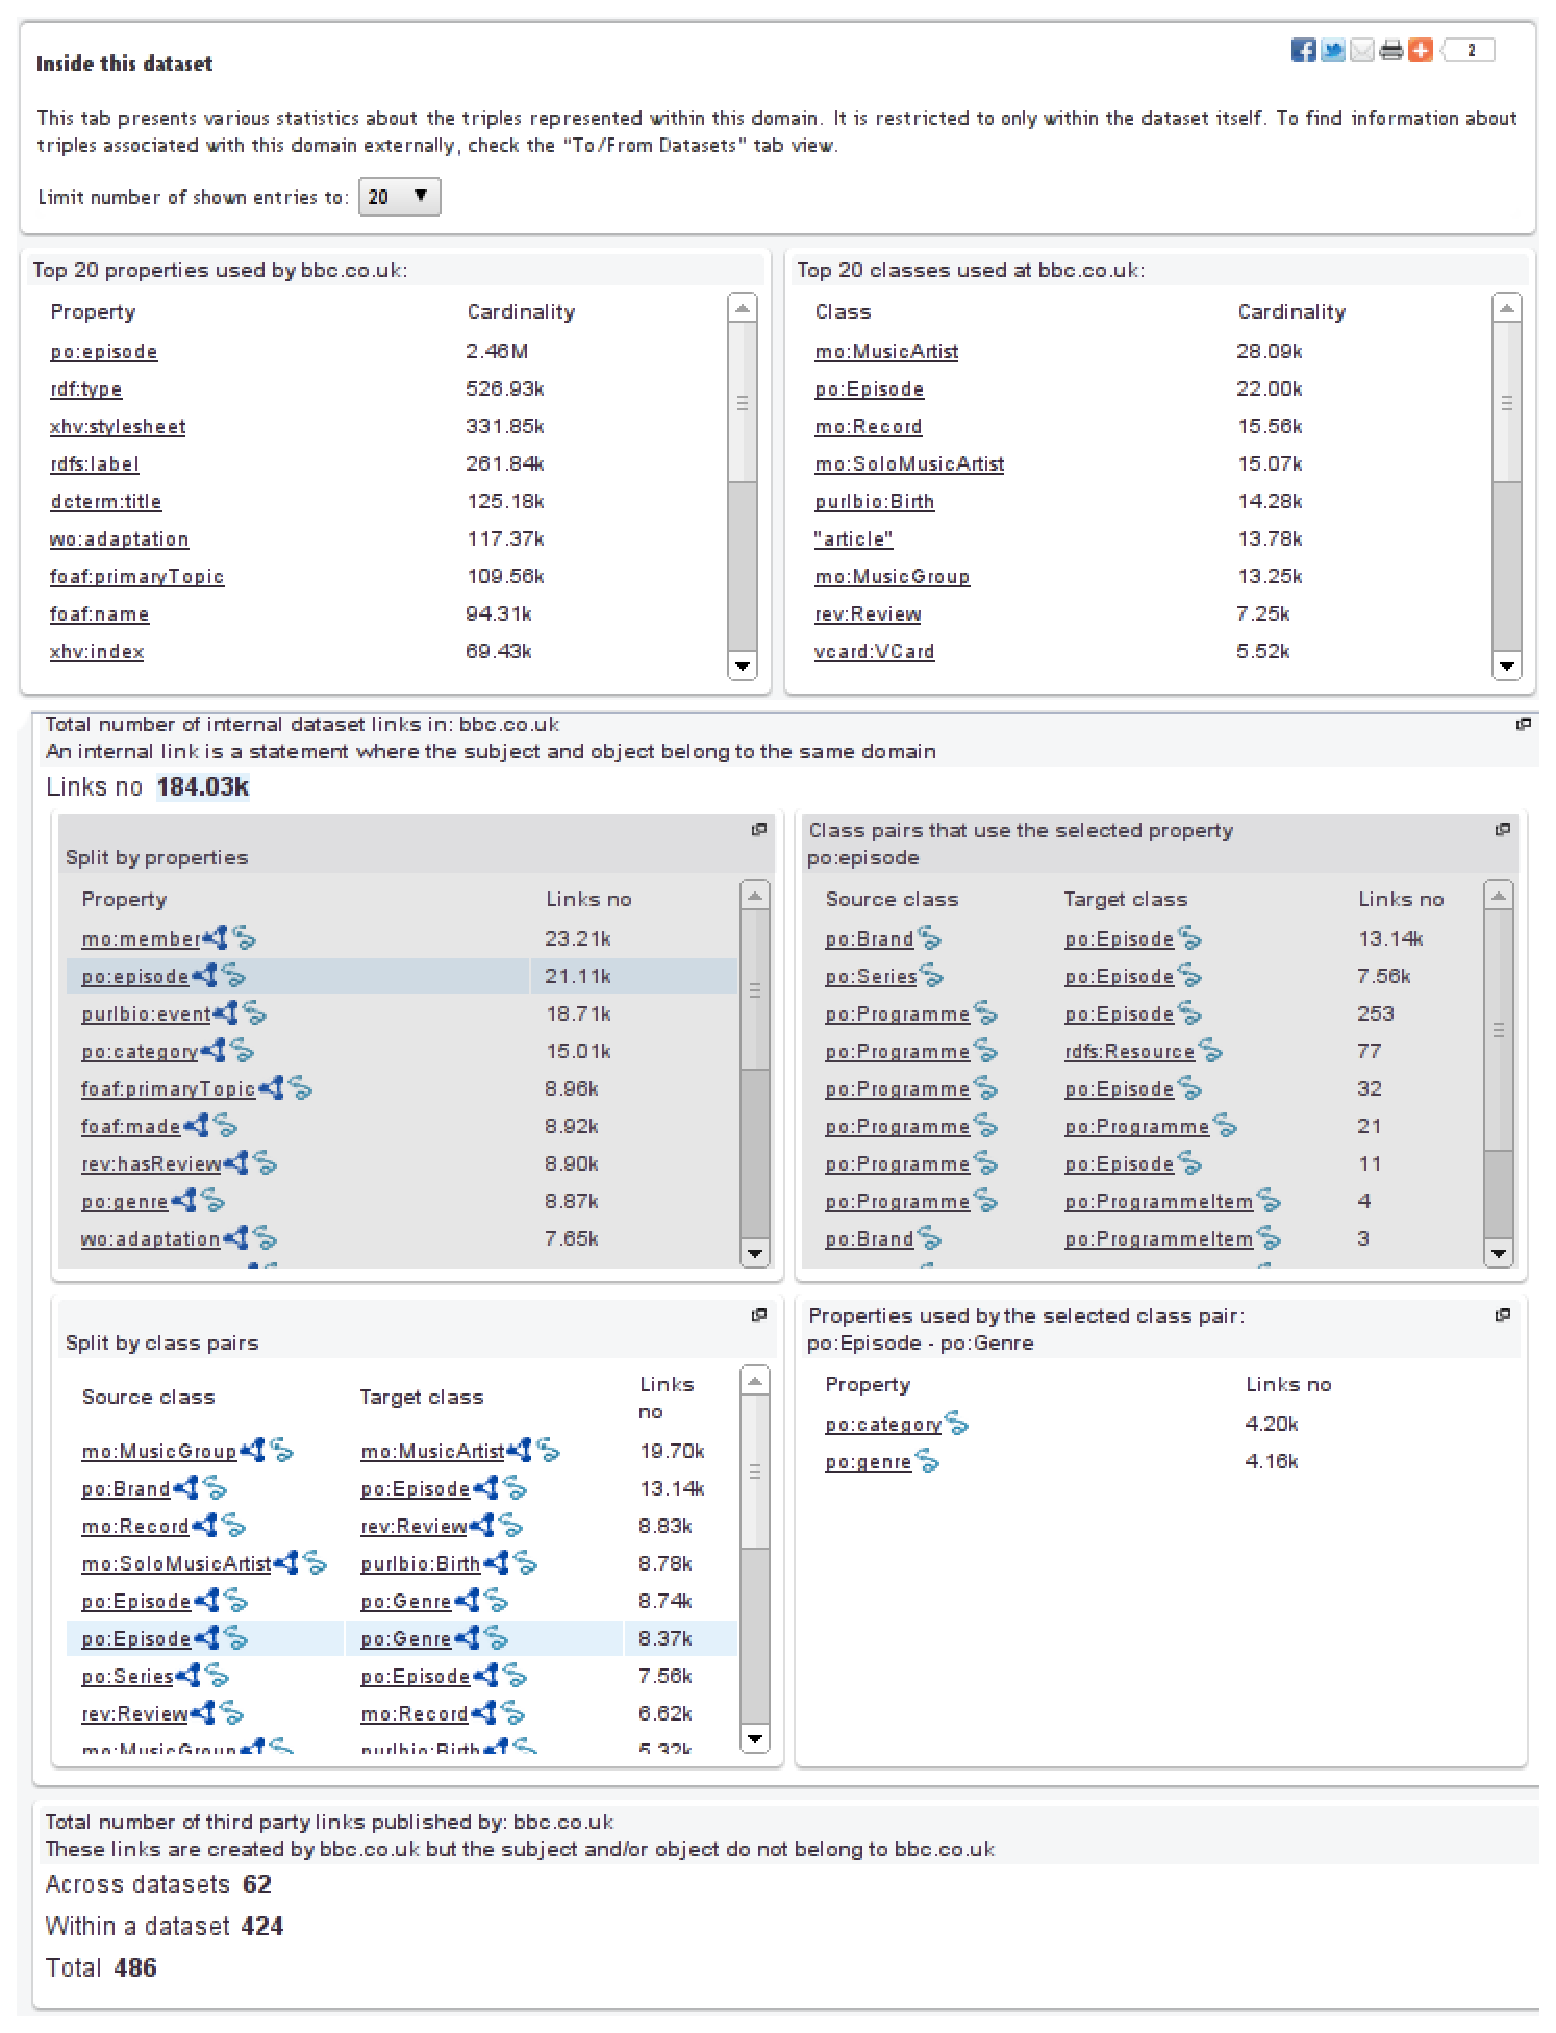
\includegraphics[scale=1]{images/applications/insideThisDataset.eps}
        }
    \end{figure}
}

\frame{
    \frametitle{To/From the Dataset View}
    \begin{figure}
        \centering
        \resizebox{!}{.8\textheight}{
            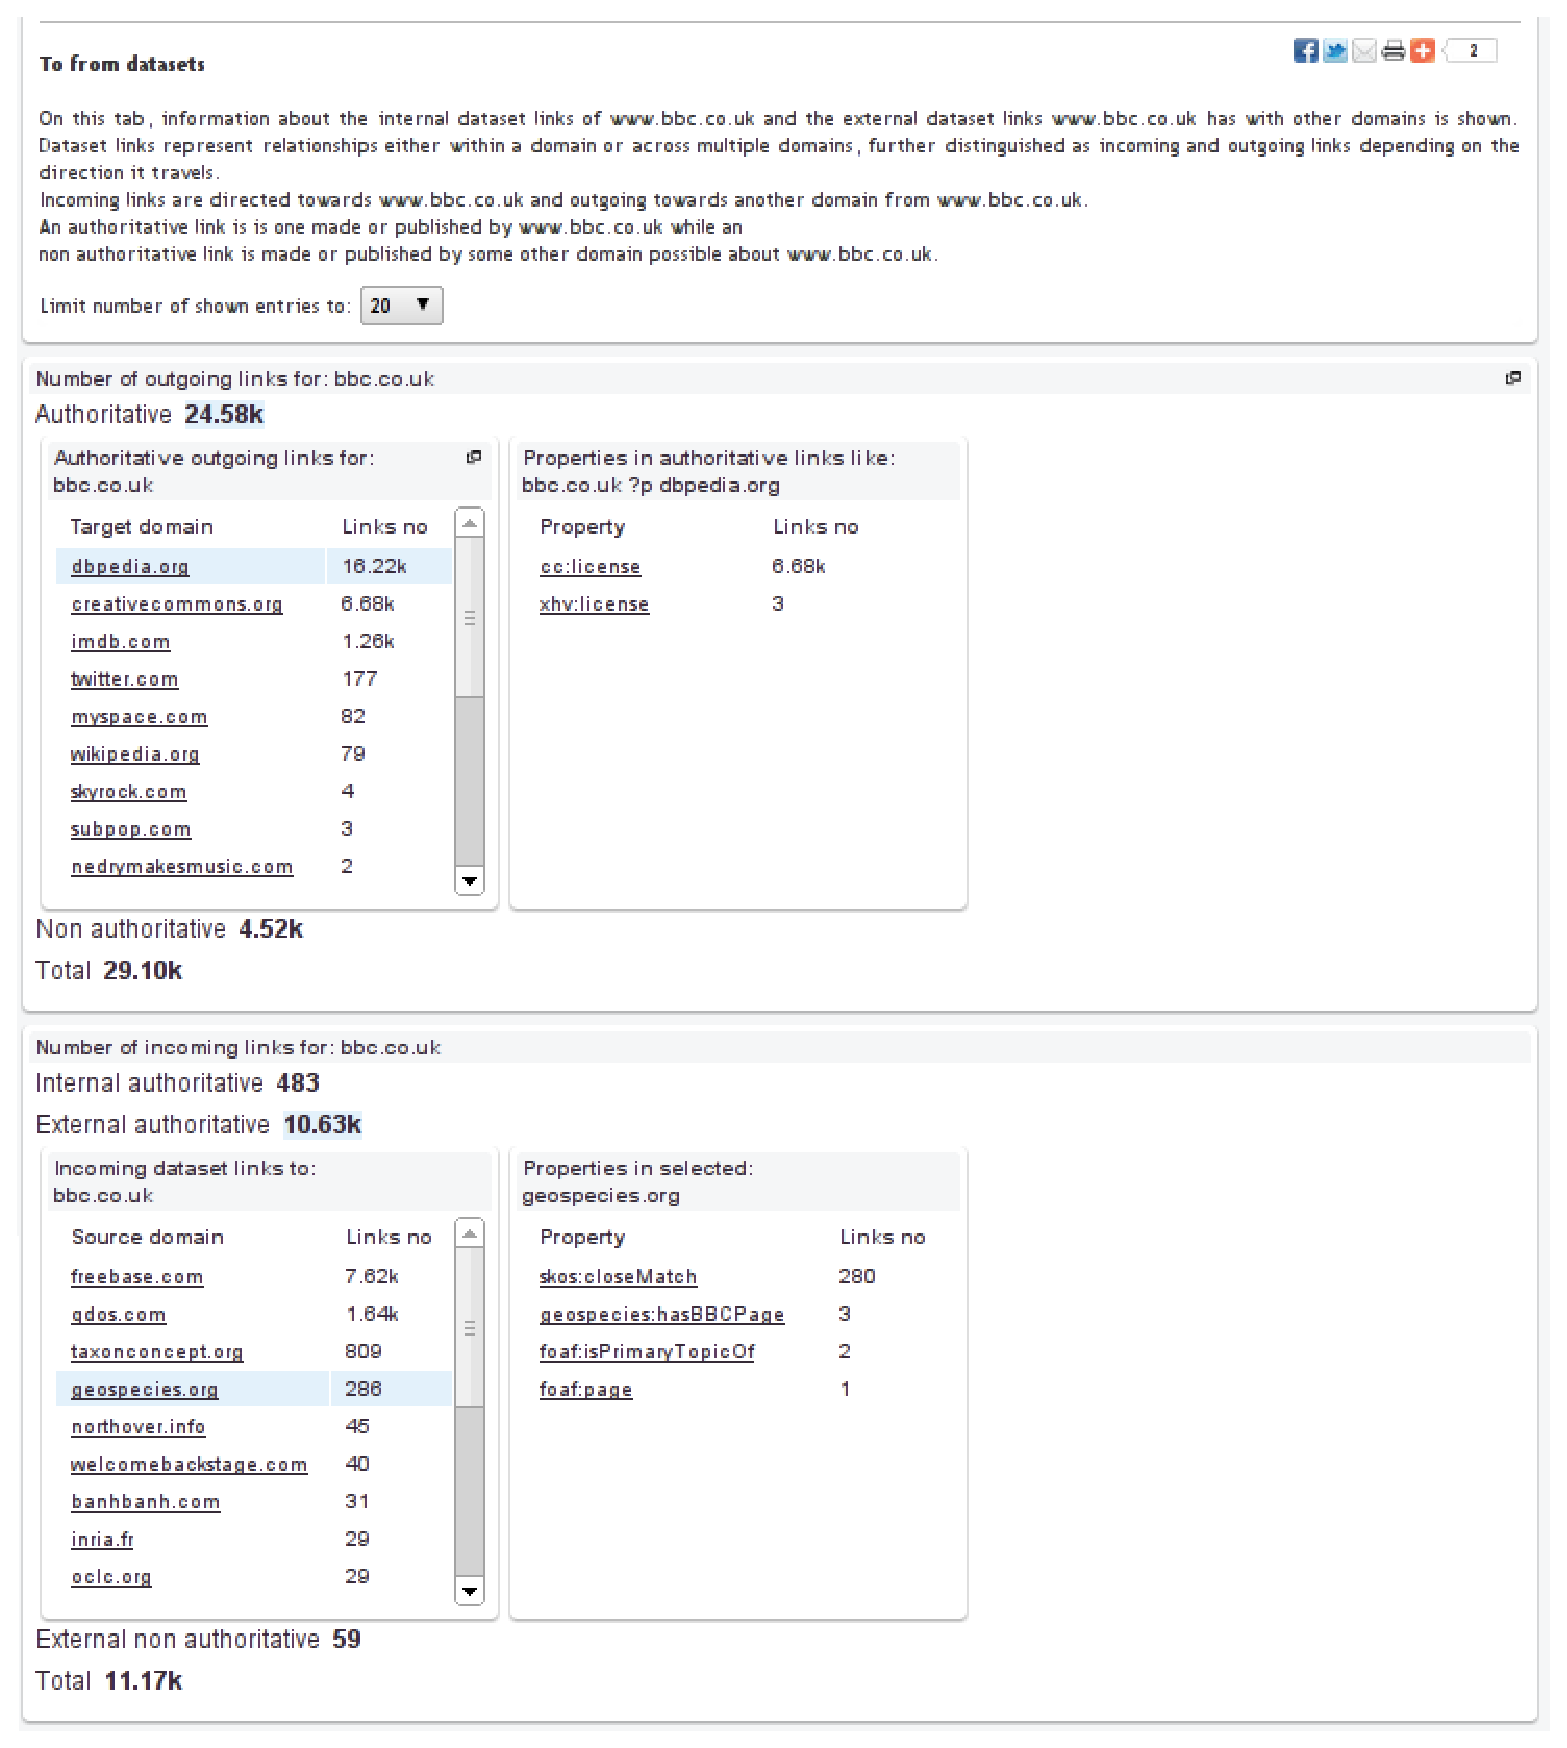
\includegraphics[scale=1]{images/applications/toFromDataset.eps}
        }
    \end{figure}
}

\frame{
    \frametitle{Third-party Links View}
    \begin{figure}
        \centering
        \resizebox{!}{.7\textheight}{
            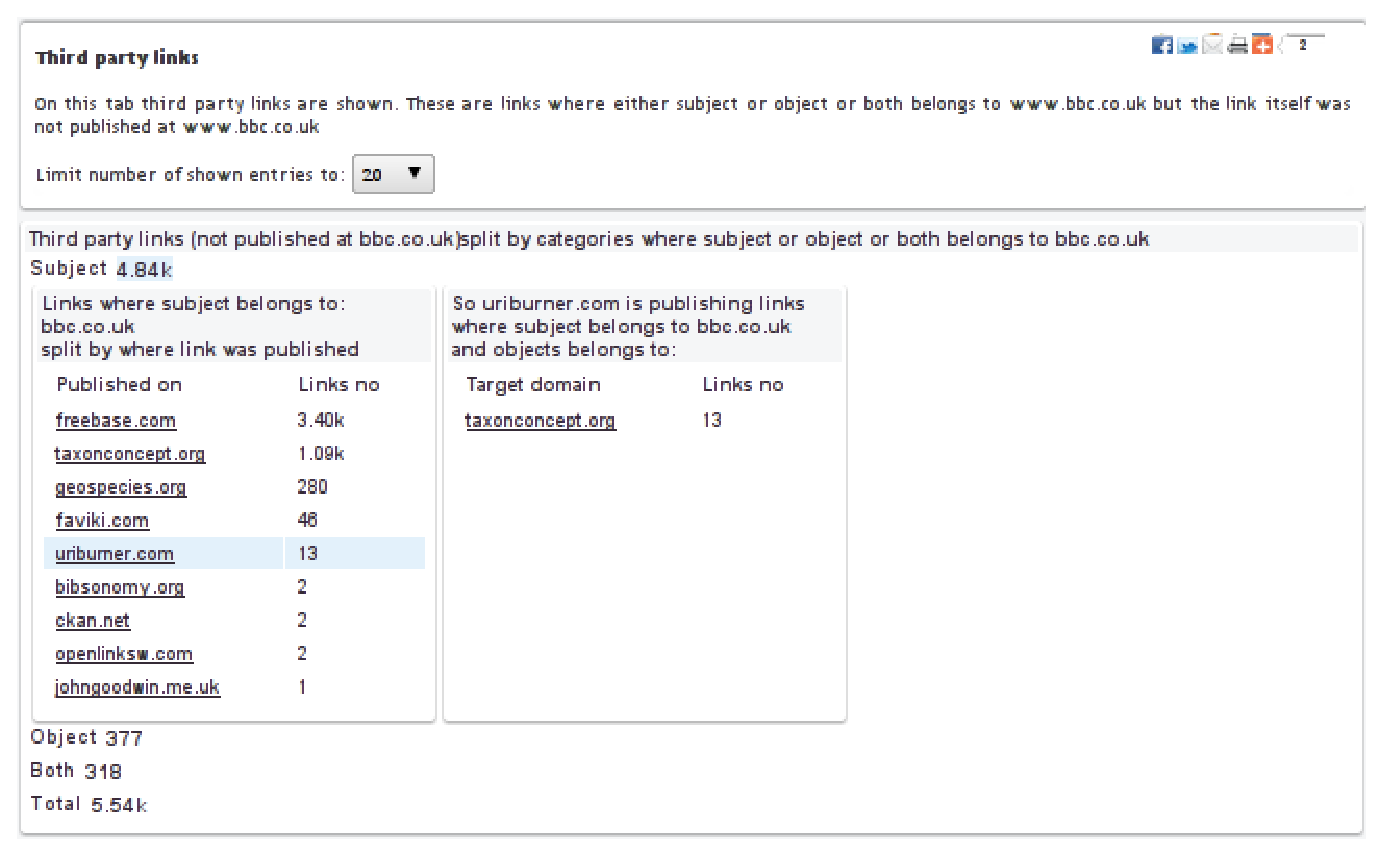
\includegraphics[scale=1]{images/applications/thirdPartyLinks.eps}
        }
    \end{figure}
}

%% vim: et:sw=4
